\documentclass[11pt,a4paper,titlepage, ngerman]{article}

\usepackage[utf8]{inputenc}	% Diese Pakete sind
\usepackage[T1]{fontenc}		% für die Verwendung 
\usepackage{ngerman}			% von Umlauten im tex-file
\usepackage{lmodern}			% Schriftart, die am Bildschirm besser lesbar ist
\usepackage{graphicx}			% Zum Einbinden von Formeln
\usepackage{url}					% Zur Darstellung von Webadressen
\usepackage{siunitx}
\usepackage{amsmath}			% für equation*
\usepackage{subcaption}
\usepackage{wrapfig}

\begin{document}
	\setlength{\parindent}{0em} 
	
	\begin{titlepage}
		\centering
		{\scshape\LARGE Versuchsbericht zu \par}
		\vspace{1cm}
		{\scshape\huge S2 -- Experimentieren, und dann?\par}
		\vspace{2.5cm}
		{\LARGE Gruppe 10 Mi\par}
		\vspace{0.5cm}
		{\large Alex Oster (E-Mail: a\_oste16@uni--muenster.de) \par}
		{\large Jonathan Sigrist (E-Mail: j\_sigr01@uni--muenster.de ) \par}
		\vfill
		durchgeführt am 25.10.2017\par
		betreut von\par
		{\large Dr. Anke \textsc{Schmidt}}
		
		\vfill
		
		{\large \today\par}
	\end{titlepage}
		
	\tableofcontents
	
	\newpage
	
	\section{Einleitung}
		\label{Einleitung}
		
		
		\glqq Die Gravitationskonstante $g$ besitzt in der Stadt Münster einen Wert von \SIrange{10,5}{11}{m/s^2}.\grqq
		\\
		Zu dieser Aussage führten die Ergebnisse einer Fallgeschwindigkeitsmessung. Hierbei wurden die Geschwindigkeiten einer fallenden Metallkugel an zwei verschiedenen Punkten, mit Hilfe von Lichtschranken gemessen. Dadurch ließ sich die Fallbeschleunigung, d.h. die Gravitationskonstante, bestimmen.  
		\\
		\\
		In diesem Bericht beschäftigen wir uns damit, diese Aussage zu widerlegen.
		Dazu messen wir die Zeit von Pendelschwingungen und berechnen aus Fadenlänge und gemessener Zeit die Gravitationskonstante. Um ein möglichst genaues Ergebnis zu erhalten, führen wir mehrere Messungen mit verschiedenen Fadenlängen durch.
		
	\section{Durchführung}
		\label{Durchführung}
		
		\subsection{Versuchsaufbau}
		\label{Versuchsaufbau}
			
			Für unsere Messung haben wir eine, an einem Faden befestigte, Metallkugel verwendet. Der Faden war dabei an einer Halterung angebracht und seine Länge ließ sich beliebig einstellen.
			
					\begin{figure}[ht]
						\centering
						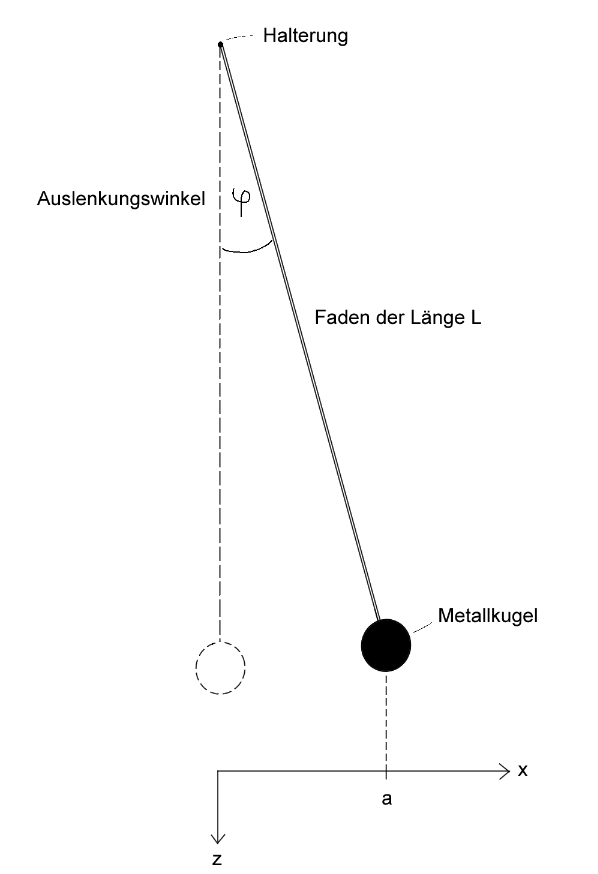
\includegraphics[scale=0.4]{Pendel.png}		
						\caption{Versuchsskizze}
						\label{fig:pendel}
					\end{figure}
			
			\newpage
			 Die Kugel wurde am Punkt $x = a$ losgelassen und wir haben die Zeit gemessen, welche die Metallkugel benötigt hat, um eine Schwingung zu durchlaufen, also bis die Metallkugel wieder bei ca. $x = a$ angekommen war. 
			
			Bei diesem Versuch verwendeten wir einen Faden der Länge $L$, kleine Auslenkungswinkel $\varphi$ und eine Metallkugel mit einen Durchmesser von \SI{3}{cm} (bzw. einem Radius von \SI{1,5}{cm}). Die Ungenauigkeiten werden in (\ref{Diskussion} Diskussion) betrachtet.
			\vspace{0.25cm}
		
		\subsection{Messung}
		\label{Messung}
			Es folgen die durchgeführten Messungen für verschiedene Fadenlängen $L$: 
			\vspace{0.25cm} 
			
			\begin{description}
				
				\item[Fadenlänge 1:]($L = \SI{111,6}{cm}$)\\ 				
				Für die erste Fadenlänge haben wir 110 Schwingungsdauern in 10er Schritten gemessen. (D.h. jeweils die Periodendauer für zehn Schwingungen auf einmal) \\
				Die durchschnittliche Zeit für eine Pendelschwingung betrug hierbei: \SI{2.134182}{s}
				
				\item[Fadenlänge 2:]($L = \SI{104,5}{cm}$)\\ 				 
				Bei dieser und der folgenden Messung haben wir nur 20 Perioden, in 5er Schritten, gemessen. Hier betrug die durchschnittliche Zeit für eine Pendelschwingung: \SI{0}{s}
				
				\item[Fadenlänge 3:]($L = \SI{86,9}{cm}$)\\ 			
				Wie auch bei der vorherigen Messung wurden hier nur 20 Schwingungen betrachtet. Dabei ergab sich, für eine Pendelschwingung, die durchschnittliche Zeit: \SI{0}{s}		
				
				\item[Fadenlänge 4:]($L = \SI{65,8}{cm}$)\\ 				
				Diese Messung und die Folgende betrachten wir 25 Perioden, ebenfalls in 5er Schritten. Die durchschnittliche Zeit für eine Pendelschwingung betrug hierbei: \SI{0}{s}
				
				\item[Fadenlänge 5:]($L = \SI{116,3}{cm}$)\\ 				
				Hier erhalten wir für eine Pendelschwingung die durchschnittliche Zeit: \SI{0}{s}
				
				\item[Fadenlänge 6:]($L = \SI{92,6}{cm}$)\\ 				
				Da wir bei den letzten vier Messungen nicht viele Schwingungen betrachtet haben, haben wir für die sechste Fadenlänge noch einmal 100 Schwingungsdauern gemessen. Dabei haben wir eine Länge $L$ gewählt, die circa \SI{20}{cm} von der ersten abwich, um mehrere Werte für \glqq deutlich\grqq unterschiedliche Längen $L$ zu erhalten. 
				Hierbei betrug die durchschnittliche Zeit für eine Pendelschwingung: \SI{0}{s}
				
			\end{description}
		
	\section{Diskussion}	
		\label{Diskussion}		
		
		
			
\end{document} 